\chapter{Information Bottleneck*}
\begin{figure}[htbp]
    \centering
    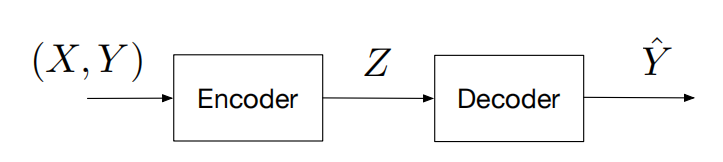
\includegraphics[width=0.8\textwidth]{./figures/chapter9/AE.png}
\end{figure}
$(X, Y)$: Source input, $Z$: extracted features, $\hat{Y}$: predicted label. \\
Information complexity: $I(X;Z)$, information utility: $I(Z;Y)$. \\
Trade-off: $L = \min\limits_{p(z|x)} I(X;Z) - \beta I(Z;Y)$, 其中后半部分是为了防止过拟合.

\begin{figure}[htbp]
    \centering
    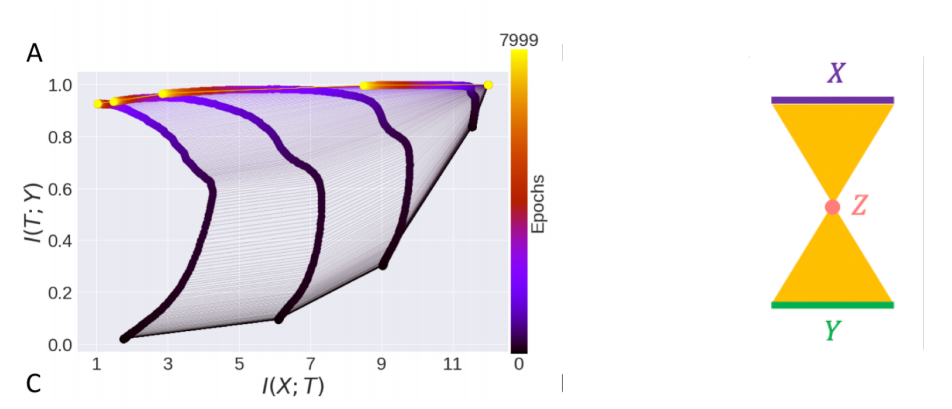
\includegraphics[width=0.8\textwidth]{./figures/chapter9/bottleneck.png}
\end{figure}
若将 Encoder 和 Decoder 都换成 neural network, 则会出现上图的现象. \\
从左往右四条线是网络的深度, 在同一层中, 互信息会先增大后降低. 感性理解: 学习的过程中需要先把书学厚, 然后再学薄.

\begin{figure}[htbp]
    \centering
    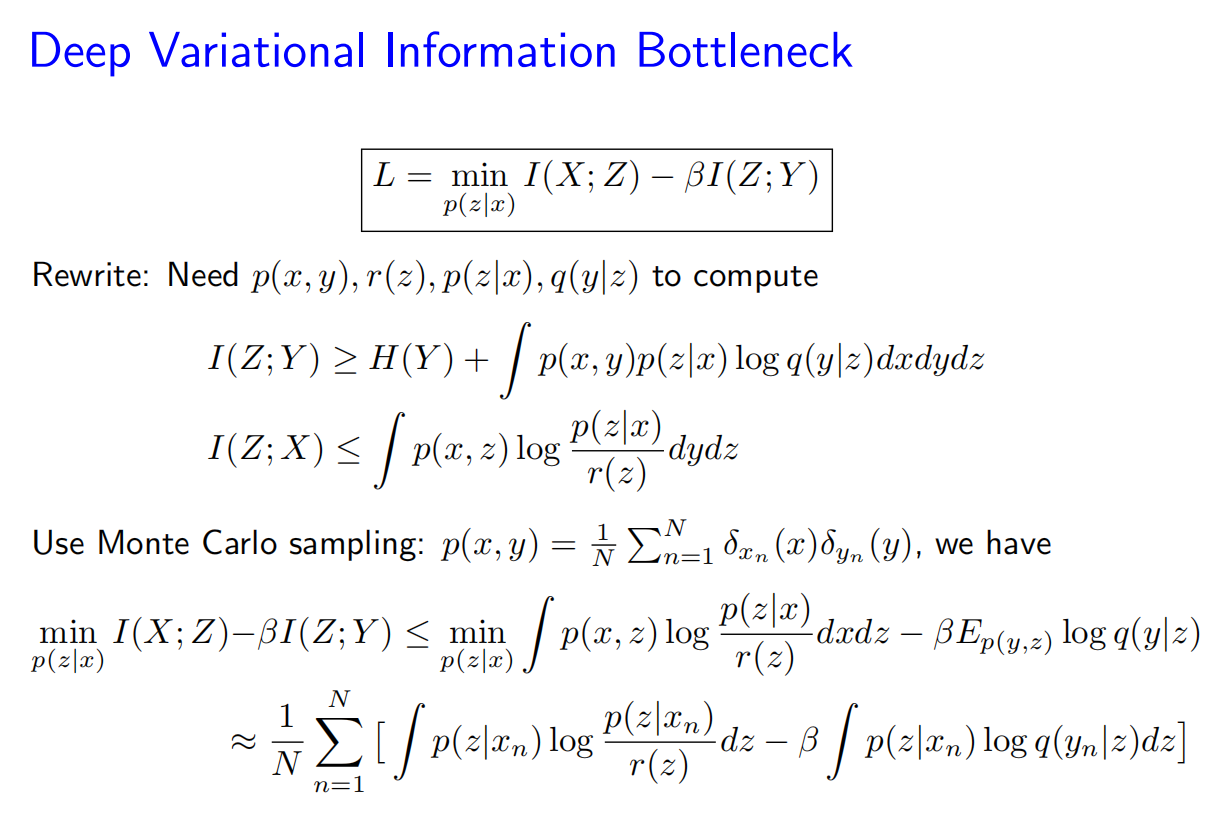
\includegraphics[width=\textwidth]{./figures/chapter9/result.png}
\end{figure}
$p(z|x)$为训练得到的encoder, $p(y|z)$为训练得到的decoder. $p(x,y)$ 无法直接得到, 用 Monte Carlo从样本中采样估计. \\
VAE中重参数化, ELBO等 details in PPT.